\chapter{Arhitektura i dizajn sustava}
		
		\textbf{\textit{dio 1. revizije}}\\

		\textit{ Potrebno je opisati stil arhitekture te identificirati: podsustave, preslikavanje na radnu platformu, spremišta podataka, mrežne protokole, globalni upravljački tok i sklopovsko-programske zahtjeve. Po točkama razraditi i popratiti odgovarajućim skicama:}
	\begin{itemize}
		\item 	\textit{izbor arhitekture temeljem principa oblikovanja pokazanih na predavanjima (objasniti zašto ste baš odabrali takvu arhitekturu)}
		\item 	\textit{organizaciju sustava s najviše razine apstrakcije (npr. klijent-poslužitelj, baza podataka, datotečni sustav, grafičko sučelje)}
		\item 	\textit{organizaciju aplikacije (npr. slojevi frontend i backend, MVC arhitektura) }		
	\end{itemize}

	
		

		

				
		\section{Baza podataka}
			
			
			
		Za potrebe naseg sustava koristit cemo relacijsku bazu podataka koja svojom strukturom olaksava modeliranje stvarnog svijeta. Gradivna jedinka baze je relacija, odnosno tablica koja je definirana svojim imenom i skupom atributa. Zadaca baze podataka je brza i jednostavna pohrana, izmjena i dohvat podataka za daljnju obradu.
Baza podataka ove aplikacije sastoji se od sljedecih entiteta: 
\begin{itemize}
		\item Korisnik
		\item Uloge
		\item Donacija
		\item Krv
		\item Potrošnja
	\end{itemize}

		
			\subsection{Opis tablica}
			

				Svaku tablicu je potrebno opisati po zadanom predlošku. Lijevo se nalazi točno ime varijable u bazi podataka, u sredini se nalazi tip podataka, a desno se nalazi opis varijable. Svjetlozelenom bojom označite primarni ključ. Svjetlo plavom označite strani ključ
				
				
				\begin{longtblr}[
					label=none,
					entry=none
					]{
						width = \textwidth,
						colspec={|X[6,l]|X[6, l]|X[20, l]|}, 
						rowhead = 1,
					} %definicija širine tablice, širine stupaca, poravnanje i broja redaka naslova tablice
					\hline \multicolumn{3}{|c|}{\textbf{Korisnik}}	 \\ \hline[3pt]
					\SetCell{LightGreen}Korisničko ime & VARCHAR & ime pomocu kojeg se korisnik logina (jednako donorid za donore) \\ \hline
					lozinka	& VARCHAR &  lozinka za login 	\\ \hline 
					email & VARCHAR & email na koji korisniku dolaze korisne informacije  \\ \hline 
					broj mobitela & INT	&  broj na koji korisniku dolaze korisne infromacije		\\ \hline
					ime & VARCHAR	&  ime korisnika		\\ \hline 
					prezime & VARCHAR	& prezime korisnika	\\ \hline 
                     godina rodenja & INT	&  godina rodenja	\\ \hline
                     mjesto prebivanja & VARCHAR	&  mjesto stanovanja		\\ \hline
                     zdravstveni podaci & VARCHAR	&  	kratki opis zdravstvenog stanja	\\ \hline
					\SetCell{LightBlue} uloga id	& INT &  označuje da li je korisnik admin, djelatnik ili donor 	\\ \hline 
				\end{longtblr}
				
				\begin{longtblr}[
					label=none,
					entry=none
					]{
						width = \textwidth,
						colspec={|X[6,l]|X[6, l]|X[20, l]|}, 
						rowhead = 1,
					} %definicija širine tablice, širine stupaca, poravnanje i broja redaka naslova tablice
					\hline \multicolumn{3}{|c|}{\textbf{Uloge}}	 \\ \hline[3pt]
					\SetCell{LightGreen}Uloga id & INT	& označuje id uloge (admin, djelatnik ili donor)\\ \hline
					uloga name	& VARCHAR & ime uloge(donor,admin...)  	\\ \hline 
				\end{longtblr}
				
				\begin{longtblr}[
					label=none,
					entry=none
					]{
						width = \textwidth,
						colspec={|X[6,l]|X[6, l]|X[20, l]|}, 
						rowhead = 1,
					} %definicija širine tablice, širine stupaca, poravnanje i broja redaka naslova tablice
					\hline \multicolumn{3}{|c|}{\textbf{Donacija}}	 \\ \hline[3pt]
					\SetCell{LightGreen}Korisničko_ime & VARCHAR & korisničko ime (donorId) korisnika koji je donirao \\ \hline
					\SetCell{LightGreen}datum & DATE & datum donacije \\ \hline

					Mjesto	& VARCHAR & mjesto donacije	\\ \hline 
					Uspješnost	& INT & 0 za neuspješnu, 1 za uspješnu donaciju krvi  	\\ \hline 
					
					\SetCell{LightBlue} Korisničkoime djelatnika	& VARCHAR &  korisničko ime djelatnika koji je primio donaciju 	\\ \hline 
				\end{longtblr}
				
				\begin{longtblr}[
					label=none,
					entry=none
					]{
						width = \textwidth,
						colspec={|X[6,l]|X[6, l]|X[20, l]|}, 
						rowhead = 1,
					} %definicija širine tablice, širine stupaca, poravnanje i broja redaka naslova tablice
					\hline \multicolumn{3}{|c|}{\textbf{Krv}}	 \\ \hline[3pt]
					\SetCell{LightGreen}ime krvne grupe & VARCHAR & (A+,A-,AB+,B-...) \\ \hline
					gornja granica & INT & gornja granica dopuštene količine krvi u jedinicama\\ \hline

					donja granica	& INT & donja granica dopuštene količine krvi u jedinicama  	\\ \hline 
					trenutna zaliha	& INT &  trenutna zaliha konkretne krve grupe u jedinicama 	\\ \hline 
					
					
				\end{longtblr}
				
				\begin{longtblr}[
					label=none,
					entry=none
					]{
						width = \textwidth,
						colspec={|X[6,l]|X[6, l]|X[20, l]|}, 
						rowhead = 1,
					} %definicija širine tablice, širine stupaca, poravnanje i broja redaka naslova tablice
					\hline \multicolumn{3}{|c|}{\textbf{Potrošnja}}	 \\ \hline[3pt]
					\SetCell{LightGreen}ime krvne grupe & VARCHAR & ime krvne grupe \\ \hline
					\SetCell{LightGreen}timestampPotrošnje & DATETIME & timestamp potrošnje \\ \hline

					količina 	& INT &  broj jedinica koji su se potrošili 	\\ \hline 
					
					\SetCell{LightBlue} korisničko ime djelatnika	& VARCHAR &  korisničko ime djelatnika koji je inicirao slanje krvi bolnici	\\ \hline 
				\end{longtblr}
				
			
			\subsection{Dijagram baze podataka}
				\begin{figure}[H]
	\centering
	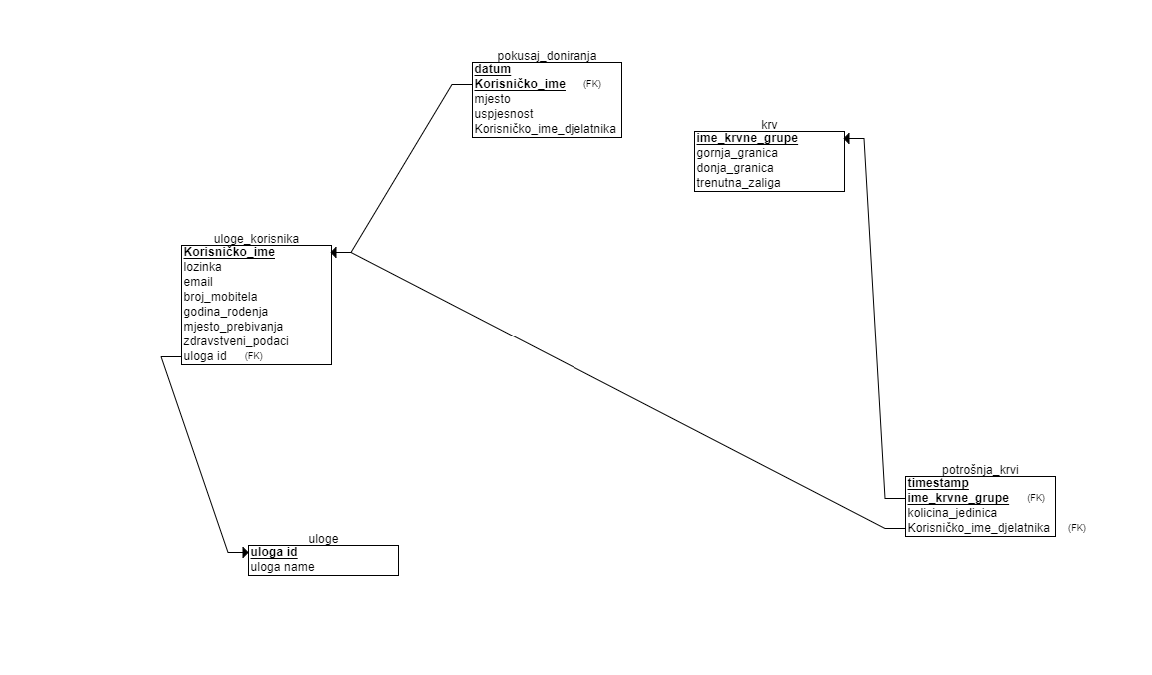
\includegraphics[width=\textwidth, scale=2.0]{dijagrami/dijagram_baze.png}
	\caption{E-R dijagram baze podataka UC8}
	\label{fig:dijagram_baze}
\end{figure}
			\eject
			
		\section{Dijagram razreda}
		
			\textit{Potrebno je priložiti dijagram razreda s pripadajućim opisom. Zbog preglednosti je moguće dijagram razlomiti na više njih, ali moraju biti grupirani prema sličnim razinama apstrakcije i srodnim funkcionalnostima.}\\
			
			\textbf{\textit{dio 1. revizije}}\\
			
			\textit{Prilikom prve predaje projekta, potrebno je priložiti potpuno razrađen dijagram razreda vezan uz \textbf{generičku funkcionalnost} sustava. Ostale funkcionalnosti trebaju biti idejno razrađene u dijagramu sa sljedećim komponentama: nazivi razreda, nazivi metoda i vrste pristupa metodama (npr. javni, zaštićeni), nazivi atributa razreda, veze i odnosi između razreda.}\\
			
			\textbf{\textit{dio 2. revizije}}\\			
			
			\textit{Prilikom druge predaje projekta dijagram razreda i opisi moraju odgovarati stvarnom stanju implementacije}
			
			
			
			\eject
		
		\section{Dijagram stanja}
			
			
			\textbf{\textit{dio 2. revizije}}\\
			
			\textit{Potrebno je priložiti dijagram stanja i opisati ga. Dovoljan je jedan dijagram stanja koji prikazuje \textbf{značajan dio funkcionalnosti} sustava. Na primjer, stanja korisničkog sučelja i tijek korištenja neke ključne funkcionalnosti jesu značajan dio sustava, a registracija i prijava nisu. }
			
			
			\eject 
		
		\section{Dijagram aktivnosti}
			
			\textbf{\textit{dio 2. revizije}}\\
			
			 \textit{Potrebno je priložiti dijagram aktivnosti s pripadajućim opisom. Dijagram aktivnosti treba prikazivati značajan dio sustava.}
			
			\eject
		\section{Dijagram komponenti}
		
			\textbf{\textit{dio 2. revizije}}\\
		
			 \textit{Potrebno je priložiti dijagram komponenti s pripadajućim opisom. Dijagram komponenti treba prikazivati strukturu cijele aplikacije.}
